% \bibliography{../src/bibliography}

This chapter introduces a neural Conditional Random Field (CRF) parser that can be used as an alternative proposal distribution for the approximate marginalization of the RNNG. The model is a span-factored CRF that independently predicts scores for labeled spans over the sentence using neural networks. The scores then interact in a chart-based dynamic program, giving a compact description of the probability distribution over parses. This approach combines the efficient exact inference of chart-based parsing, the rich nonlinear features of neural networks, and the global training of a CRF. The chart-based approach allows efficient exact inference alowing for exact decoding and global sampling while the neural features can be complex and can condition on the entire sentence. The CRF training objective [...something about receiving information about all substructures...]. The parser is an adaptation of the chart-based parser introduced in \citet{stern2017minimal} to global CRF training. \citet{stern2017minimal} train the model with a margin-based objective, but our interest primary in this model is as a proposal distribution, which requires probabilistical training.

In this chapter:
\begin{itemize}
  \item I present the parser and describe how it is an adaptation of earlier log-linear and neural crf parsing \citep{finkel2008crf,klein2015crf} and the maximum margin trained parser of \citet{stern2017minimal}.
  \item I show how the several inference problems of interest can be solved exactly: prediction, entropy, sampling.
  \item We train the parser in a supervised fashion and show it's adequacy as a parser.
  \item We invesitage the kind of samples that are obtained from this parser, and evaluate how they affect the approximate inference in the RNNG.
\end{itemize}


\section{Model}
The model is a CRF factored over the labeled spans that form a tree. We write $\y_a = (A, i, j) }$ for a span $\langle x_{i+1}, \dots, \x_j \rangle$ labeled by  and $A$, and consider a tree $\y$ as a collection of these parts:
\begin{align}
  \y = \{ \y_a \}_{a=1}^A.
\end{align}
We define the score $\Psix, \y)$ of tree as the product of nonnegative local potentials $\psi(\x, \y_a) \geq 0$:
\begin{align}
  \Psi(\x, \y) = \prod_{a=1}^A \psi(\x, \y_a).
\end{align}
 The function $\psi$ scores each span seperately, but conditional on the entire sentence. The probability of a tree is the globally normalized score of the tree:
\begin{align}
  \label{eq:crf-model}
  p(\y \mid \x) &= \frac{1}{Z(\x)} \prod_{a=1}^A \psi(\x, \y_a),
\end{align}
where
\begin{align*}
  Z(\x) = \sum_{ \y \in \yieldx } \prod_{a=1}^A \psi(\x, \y_a)
\end{align*}
is the normalizing constant that sums over all the possible parse trees that ensures that the probability distribution sums to 1. This normalizing constant can be computed efficiently with the inside algorithm.

By factorizing a tree over labeled spans we make an even stronger assumption than that typically made by factorizating over anchored context-free rules\footnote{\cf table \ref{tab:spans-rules} for the different conceptions.}. This way, the potential function has no access to information about the direct substructure under the node, such as the child nodes and their split point. The function can thus rely less on the local tree structure and must thus rely more on the surface features of input sentence. This factorization will, however, greatly reduce the size of the state-space of the dynamic programs, speeding up training and inference, and the burden of the feature function will be carried by a rich neural network parametrization. Together, this will make the parser fast and very effective.

\section{Parametrization}
The scoring function $\psi$ is implemented with neural networks following the design of the minimal scoring function of \citet{stern2017minimal}. The local potentials can only make minimal use of structural information, as we argued above, but they can depend on the entire sentence. This suggest the use of RNN encodings. The representation of a span $(i, j)$ is the concatenation of the difference between forward and backward vectors
\begin{align}
  \label{eq:potential-function}
  \vecs_{ij} = [\fw_j - \fw_i; \bw_i - \bw_j],
\end{align}
illustrated in figure \ref{fig:span-feature}. The score for a label $A$ is computed from this vector using a feedforward network.
\begin{align}
  \log \psi(\x, \y_a) = \Big[ \ff( \vecs_{ij} ) \Big]_{A}.
\end{align}
This architecture is rightly called minimal, but it works surprisingly well: \citet{stern2017minimal} experiment with more elaborate functions based on concatenation of vectors (a strict superset of the minus approach) and biaffine scoring (inspired by \citep{dozat2016deep}), but these function improve marginally, if they do at all.

\begin{figure}
  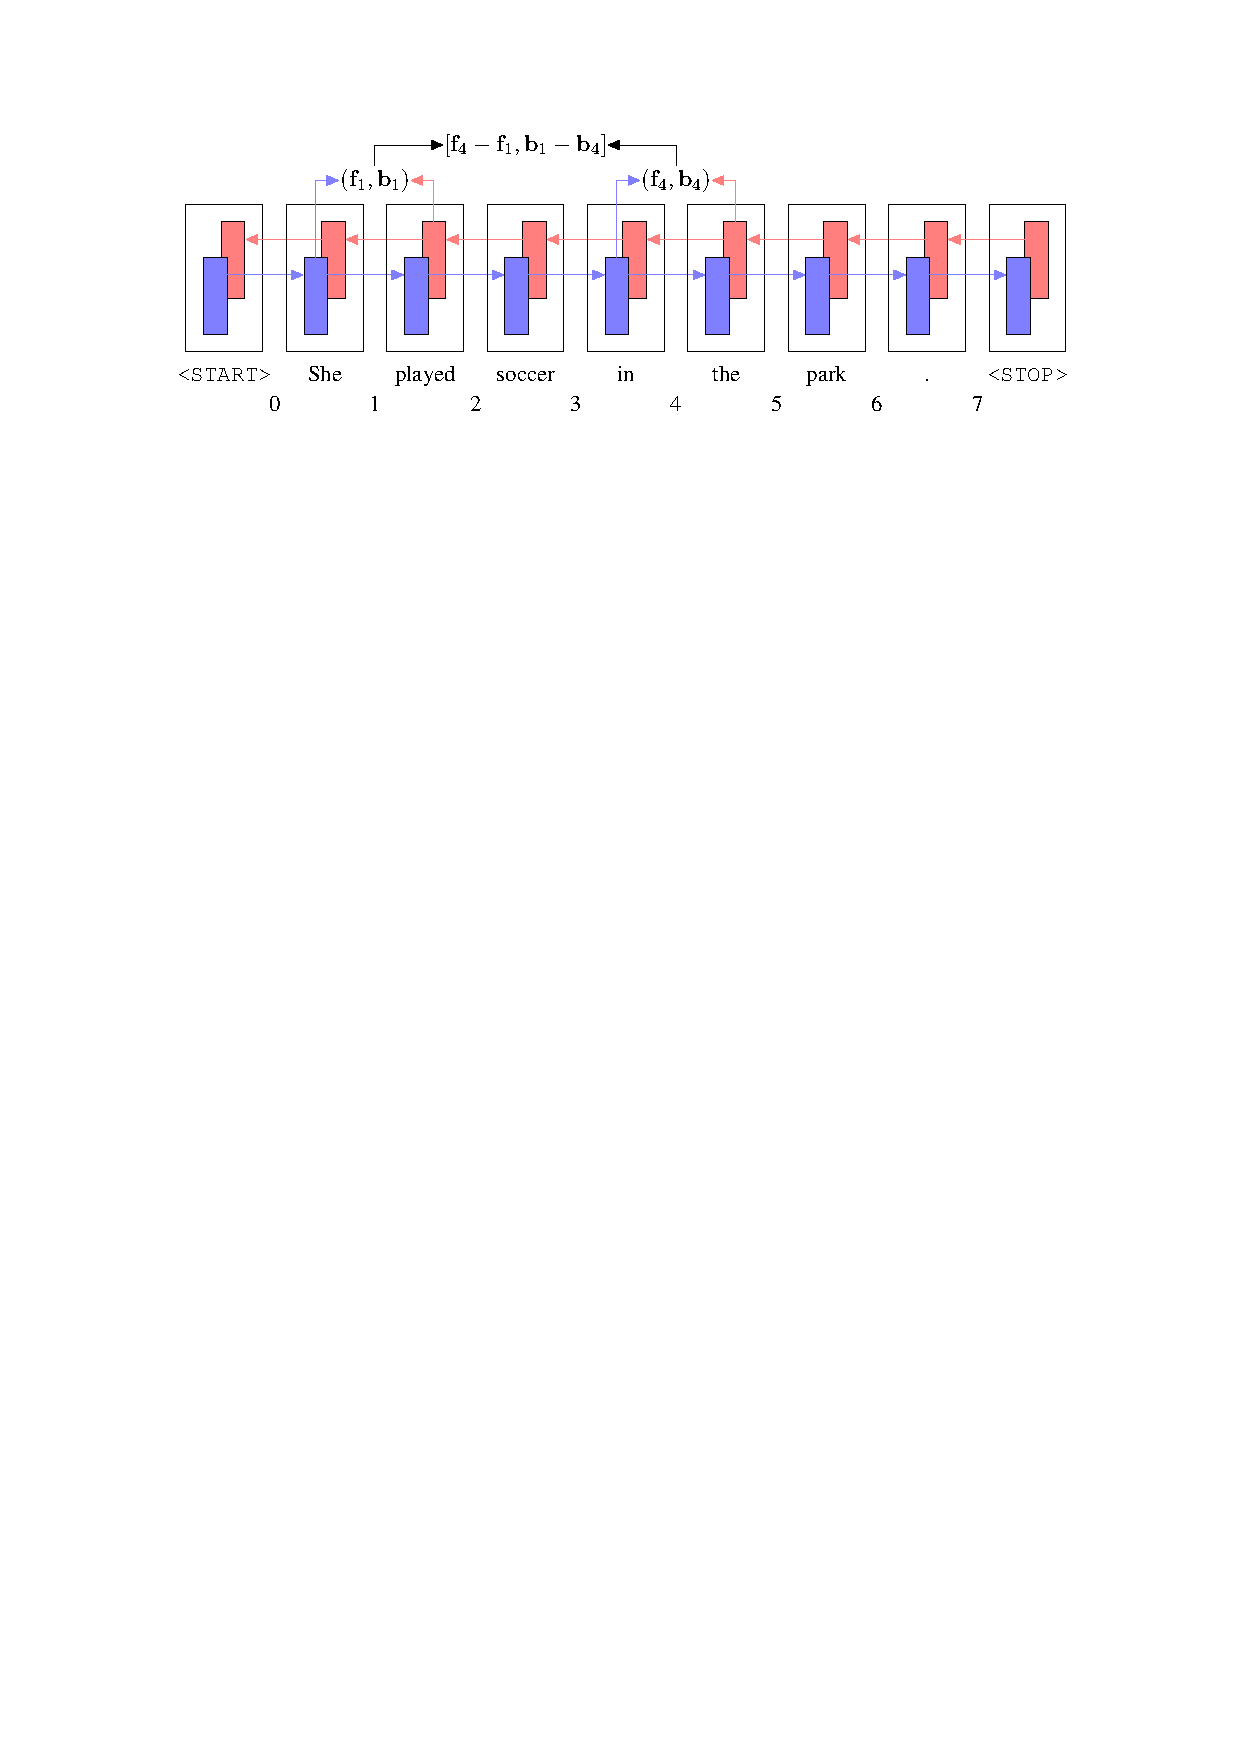
\includegraphics[width=\textwidth]{span-encoding.pdf}
  \caption{Representation for the span $(1, 4)$ computed from $\rnn$ encodings. Taken without permission from \citet{stern2018analyis}.}
  \label{fig:span-feature}
\end{figure}

\section{Inference}
Because the model is span-factored it allows efficient inference. In this section we describe efficient solutions to four related problems:
\begin{itemize}
  \item Find the best parse $\hat{ \y } = \arg \max_{\y } p(\y  \mid \x)$
  \item Compute the normalizer $Z(\x) = \sum_{ \y \in \yieldx } \prod_{ a=1 }^{ A } \psi( \x, \y_a )$.
  \item Obtain a sample $y \sim p(\cdot \mid \x)$.
  \item Compute the entropy $H(\y \mid \x)$ conditional on $\x$.
\end{itemize}
These problems are solved by variants of the inside and outside algorithms. We first describe how the quantities computed by these algorithms will be used to solve these problems, and then how these are computed.

\subsection{Quantities}
For each labeled span $(A, i, j)$, we define the inside value $\alpha(A, i, j)$ as the sum of potentials of all trees that are rooted in node $A$ with leaves $x_{i+1} \dots x_j$. We define the outside value $\beta(A, i, j)$ as the sum over potentials of all trees with leaves $x_1 \dots x_i A x_{j+1} \dots x_n$, where the nonterminal $A$ is treated as a leaf that is not expanded. These values sum over complementary sets that together make up all parses of $\x$.

% This can best be illustrated by figure \ref{fig:inside-tree} that introduces the notion of an \textit{inside tree} and an \textit{outside tree}. The inside value is the sum over the potentials of inside trees, and the outside value is the sum over all outside trees.

We then define the quantity $\mu(A, i, j)$ as the sum of all parses of $\x$ that contain nonterminal $\y_a = (A, i, j)$:
\begin{align*}
  \mu(i, j, \ell)
    &\defeq \sum_{ \substack{ \y \in \yieldx \\ \y_a \in \y } } \psi(\x, \y_a),
\end{align*}
and note that under this these definition we have the result
\begin{align}
  \mu(A, i, j) &= \alpha(A, i, j) \beta(A, i, j).
\end{align}
Given these quantities, we can directly solve three problems described above.

\paragraph{Normalizer}
The normalizer is the inside value at the root node
\begin{align}
  Z(\x) = \alpha(\text{S}^{\dagger}, 0, n).
\end{align}
This follows from the definition of the inside algorithm: $\alpha(\text{S}^{\dagger}, 0, n)$ is the sum of potentials of all trees rooted in $\text{S}^{\dagger}$ that span words $x_1 \dots x_n$.

\paragraph{Node marginals}
Suppose we are sampling parses $\y$ for $\x$ from the model $p$. The probability that the parse contains labeled span $\y_a = (A, i, j)$ is called the marginal probability of $\y_a$, and is computed as
\begin{align}
  P( (A, i, j) \in Y \mid X = \x ) = \frac{\alpha(A, i, j) \cdot \beta(A, i, j)}{Z(\x)}.
\end{align}

\paragraph{Entropy}
The entropy of the distribution over parses can be computed efficiently, using the node marginals. We derive
\begin{align*}
  H(P_{Y \vert X = x})
    &= - \sum_{ \y \in \yieldx } p(\y \mid \x) \log p(\y \mid \x)  \\
    &= \log Z(\x) - \sum_{ \y \in \yieldx } p(\y \mid \x) \sum_{\y_a \in \y} \log \psi(\x, \y_a)  \\
    &= \log Z(\x) - \sum_{ \y \in \yieldx } p(\y \mid \x) \sum_{ a \in \mathcal{A}(x) } \indicator_{\y}(a) \log \psi(\x, a)  \\
    &= \log Z(\x) - \sum_{ a \in \mathcal{A}(x) } \log \psi(\x, a)  \sum_{ \y \in \yieldx } \indicator_{\y}(a) p(\y \mid \x)  \\
    &= \log Z(\x) - \sum_{ a \in \mathcal{A}(x) } \log \psi(\x, a)  \mu(a \mid \x)  \\
    &=  \log Z(\x) - \expect_{ \mu } \Big[ \log \psi(\x, a) \Big]  \\
\end{align*}

\paragraph{Parse}
The best parse can be obtained with the Viterbi algoritm, which is an instance of the inside algorithm. The viterbi algorithm replaces the sum operator of the inside algorithmm with $\max$: at each node this selects the best substructure instead of summing over all of them.

\subsection{Inside recursion}
  The inside algorithm computes the quantities $\alpha(A,i,j)$ for all labels $A \in \Lambda$ and all spans $0 \leq i < j \leq n$. From the hypergraph perspecive this is the total weight under the node $v = (A, i, j)$---the sum of the weights of all directed paths incoming at $v$. This sum can be computed using the \textit{inside recursion} \citep{goodman1999semiring}.

  At the nodes that span one word, the inside value is just the weight of the unary edge
  \begin{align}
      \label{eq:inside-base}
      \alpha(A, i, i+1) = \psi(A, i, i+1)
  \end{align}
  for $A \in \Lambda$, for all $0 \leq i < n$.

  To compute $\alpha(A, i, j)$ in the general case we need to sum over all possible binary expansions $(A \to B C, i, k, j)$ for $A, B \in \Lambda$ and $i \leq k \leq j$. This corresponds to the following recursive expression that uses the inside values of the subparts:
  \begin{align*}
  \label{eq:inside}
    \alpha(A, i, j)
      &= \bigoplus_{B \in \Lambda} \bigoplus_{C \in \Lambda} \bigoplus_{k=i+1}^{j-1} \psi(A, i, j) \otimes \alpha(B,i,k) \otimes \alpha(C,k,j) \\
      &= \psi(A, i, j) \otimes \bigoplus_{k=i+1}^{j-1} \bigoplus_{B \in \Lambda} \alpha(B,i,k) \otimes \bigoplus_{C \in \Lambda} \alpha(C,k,j) \\
      &= \psi(A, i, j) \otimes \bigoplus_{k=i+1}^{j-1} S(i,k) \otimes S(k,j)
  \end{align*}
  where we've introduced the notational abbreviation
  \begin{align*}
      S(i,j) &= \bigoplus_{A \in \Lambda} \alpha(A,i,j).
  \end{align*}
  Looking at \ref{eq:inside} we can see the marginalized values $S(i, j)$ are all that are needed for the recursion. This suggest simplifying the recursion even further as
  \begin{align*}
  \label{eq:inside-simplified}
    S(i, j)
      &= \bigoplus_{A \in \Lambda} \alpha(A,i,j) \\
      % &=  \bigoplus_{A \in \Lambda} \psi(A, i, j) \otimes \bigoplus_{k=i+1}^{j-1} S(i,k) \otimes S(k,j) \\
      &= \Bigg[ \bigoplus_{A \in \Lambda} \psi(A, i, j) \Bigg] \otimes \Bigg[\bigoplus_{k=i+1}^{j-1} S(i,k) \otimes  S(k,j) \Bigg],
  \end{align*}
  where we put explicit brackets to emphasize that independence of the subproblems of labeling and splitting.

  This recursion can be solved by computing the inside value of the nodes $(i, j, A)$ in topological order, so that the values of the subparts are availlable to compute the inside values higher up.

\subsection{Outside recursion}
  The outside algorithm computes the quantities $\beta(A,i,j)$ for all labels $A \in \Lambda$ and all spans $0 \leq i < j \leq n$. For the labels spanning the entire sentence, the outside value is defined as
  \begin{align*}
    \beta(A, 0, n) =
    \begin{cases}
      0, & \text{ if } A = \text{S}^{\dagger}  \\
      1, & \text{otherwise}.
    \end{cases}
  \end{align*}
  To compute $\beta(A, i, j)$ in the general case we need to sum over all possible upward binary expansions that $A$ can be a part of, recursively making use of the outside values already computed. This means we sum over expansions $(B \to C \; A, k, i, j)$ for all labels $B$ and $C$ and left endpoints $1 \leq k < i$, and sum over expansions $(B \to A \; C, i, j, k)$ for all labels $B$ and $C$ and right endpoints $j < k \leq n$. This corresponds to the following recursive expression that uses the outside values of the superparts:
  \begin{align*}
    \beta(A, i, j)
      &= \bigoplus_{B \in \Lambda} \bigoplus_{C \in \Lambda} \bigoplus_{k=1}^{i-1} \psi(B, k, j) \otimes \alpha(C, k, i-1) \otimes \beta(B, k, j) \\
        &\qquad \oplus \bigoplus_{B \in \Lambda} \bigoplus_{C \in \Lambda} \bigoplus_{k=j+1}^{n} \psi(B, i, k) \otimes \beta(B, i, k) \otimes \alpha(C, j+1, k) \\
      &=  \bigoplus_{k=1}^{i-1}  \Bigg[ \bigoplus_{B \in \Lambda} \psi(B, k, j)  \otimes \beta(B, k, j) \Bigg] \otimes \Bigg[ \bigoplus_{C \in \Lambda} \alpha(C, k, i-1) \Bigg] \\
        &\qquad \oplus \bigoplus_{k=j+1}^{n}  \Bigg[ \bigoplus_{B \in \Lambda}  \psi(B, i, k) \otimes \beta(B, i, k) \Bigg] \otimes  \Bigg[  \bigoplus_{C \in \Lambda} \alpha(C, j+1, k) \Bigg] \\
      &=  \bigoplus_{k=1}^{i-1}  S'(k, j) \otimes S(k, i-1) \oplus \bigoplus_{k=j+1}^{n} S'(i, k) \otimes  S(j+1, k) \\
  \end{align*}
  where
  \begin{align*}
      S(i, j) &= \bigoplus_{A \in \Lambda} \alpha(A, i, j) \\
      S'(i, j) &= \bigoplus_{A \in \Lambda} \psi(A, i, j) \beta(A, i, j)
  \end{align*}

\subsection{Viterbi recursion}
Obtaining the viterbi tree and its probability is a matter of using the inside recursion with maximization instead of a sum. The score of the best tree is  computed by replacing the sum with the $\max$ in equation
\begin{align*}
\label{eq:viterbi-score}
  \nu(i,j)
    &= [ \max_{A \in \Lambda} \tilde{s}(i, j, A) ] \cdot [\max_{ k \in \{ i+1, \dots, j-1 \} } \nu(i,k) \cdot  \nu(k,j) ].
\end{align*}
Since these maximization over label and over split point is independent, we can find them seprately
\begin{align*}
\label{eq:viterbi-tree}
  \hat{A} &= \argmax_{ A \in \Lambda } \tilde{s}(i, j, A)  \\
  \hat{k} &= \argmax_{ k \in \{ i+1, \dots, j-1 \} } \nu(i, k) \cdot \nu(k, j)
\end{align*}
The best tree is then found by following back the best splits an labels from the root.

\subparagraph{Numerical concerns}
The above recursion computes the result of exponentially many additions and multiplications. This will soon run into the problem of numerical underflow and overflow. Instead, we compute these quantities in the logarithmic domain, defining the $\oplus$ as
\begin{align*}
  a \osum b = \log(e^{a} + e^{b}),
\end{align*}
and $\otimes$ as
\begin{align*}
  a \otimes b = a + b.
\end{align*}
The definition of $\oplus$ is made numerically stable by writing
\begin{align*}
  \log(e^{a} + e^{b} = a + \log(1 + e^{b-a}) = b + \log(1 + e^{a-b})
\end{align*}
and choosing expression with the smaller exponent.


\section{Experiments}
We perform three types of experiments with the CRF parser:
\begin{itemize}
  \item We show that the model is a good supervised parser. We train the model supervised on the PTB and show the f-score on the PTB test set.
  \item We evaluate the joint RNNG with samples from the CRF parser. We compare the perplexity and fscore with RNNG case.
  \item We evauluate `how good the model is' as a sampler.
\end{itemize}

\subsection{Supervised model} We investigate the following.
\begin{itemize}
  \item We have some optimization and hyperparameter choices here. The original paper uses Adam with 0.001 and a LSTM of dimension 250, which gives the model around 2.5 million parameters. For the discriminative RRNG we use SGD with 0.1, and hidden sizes of 128 gives the model around 800,000 parameters.
  \item I suggest two experiments: (1) use the default setting from \citep{stern2017minimal} and (2) use the settings for the RNNG with a hidden size to match the 800,000 parameters.
\end{itemize}

\subsection{Proposal model} We investigate the following:
\begin{itemize}
  \item We evaluate validation F-score and perplexity.
  \item We evaluate F-score with 100 samples (as many proposal trees as possible).
  \item We evaluate perplexity with varying number of samples: 1 (argmax), 10, 20, 50, 100 (default). The peplexity evaluation with the argmax prediction gives an impression of the uncertaty in the model \citep{buys2018exact}.
  \item  We perform learning rate decay and model selection based on a development score computed with the samples from the discriminative RNNG. Undecided: should we train a separate joint RNNG with CRF samples?
\end{itemize}

\subsection{Sampler} We investigate the following:
\begin{itemize}
  \item We asses the conditional entropy of the model. This is most quantitative. Recall that conditional entropy is defined as
  \begin{equation}
    \text{H}(Y|X) = \sum_{x \in \mathcal{X}} p_X(x)\text{H}(Y|X = x),
  \end{equation}
  where
  \begin{equation}
    \text{H}(Y|X = x) = - \sum_{y \in \mathcal{Y}} p_{Y|X}(y|x) \log p_{Y|X}(y|x).
  \end{equation}
  The quantity $\text{H}(Y|X = x)$ can computed exactly with the CRF parser. We estimate the quantity $\text{H}(Y|X)$ by a sum over the development dataset. For the probabilities $p_X(x)$ we use the marginalized probabilities of the joint RNNG (with samples from the CRF parser $p_{Y|X}$).
  \item We asses for some cherry picked sentences. This is more qualitative. These sentences should be difficult or ambiguous. Or they can be ungramatical when taken from the syneval dataset. We can evaluate their entropy, and the diversity of samples, for example to see if there are clear modes. We can make violinplots of the probabilities of the samples. We can compute the f-scores of the samples compared with the argmax tree.
\end{itemize}

\section{Related work}
Here I describe related work, and in particular earlier approaches to (neural) CRF-parsing.
\begin{enumerate}
  \item Of course \citep{stern2017minimal}
  \item CRFs \citep{sutton2012crf}
  \item CRF parsing with linear and nonlinear features \citep{finkel2008crf,klein2015crf}
  \item Attempts to simplify the grammar and thus the state-space of the dynamic program \citep{hall2014less}.
  \item Recent extension of \citet{stern2017minimal}, with same model but different features \citep{kitaev2018attentive}.
\end{enumerate}

\subsection{Motivation}
The model regards a constituency tree as a collection of \textit{labeled spans} over a sentence. Earlier CRF models for constituency parsing, both log-linear and neural, factorize trees over \textit{anchored rules} \citep{finkel2008crf,klein2015crf}. This puts most of the expressiveness of the model in the state space of the dynamic program, modelling interactions between subparts of the trees through their interaction in the rules, instead of at the feature level. The model in \citet{stern2017minimal} removes part of this structure, and puts more expressiveness in the input space by using rich neural feature representations conditioning on the entire sentence. The discrete interaction between the local scores remains only at level of labeled spans. This dramatically improves the speed of this model, which will become evident in the next section.

Chart based parsing has moved from grammar to features: the work of \citet{hall2014less} shows how the log-linear CRF model of \cite{finkel2008crf} can work with bare unnanotated grammars, when relying more on the surface features of the sentence, and \citet{klein2015crf} show how these surface features can be replaced with dense neural features. The work of \citep{stern2017minimal} moves one step further: the grammar is dispensed with altogether, making the model span-factored, and the scoring function is given the full power of neural networks.

Contrast this with generative parsing based on treebank grammars, where features are not available because the models are not conditional. Instead, these models rely entirely on detailed rule information: basic treebank grammars do not parse well because the rules provide too little context, and good results can only be obtained by enriching grammars. The independence assumptions in the grammar are thus typically weakened, not strengtehened. Such approaches lexicalize rules \citep{collins2003head}, annotate the rule with parent and sibling labels \citep{klein2003accurate}, or automatically learn refinements of nonterminal categories \citep{petrov2006learning}.

The closest predecessor to our model is the neural CRF parser of \citet{klein2015crf}, which predicts local potential for anchored rules using a feedfoward network. This differs from our approach in two ways. Their method requires a grammar, extracted from a treebank beforehand, whereas our approach implictly assumes all rules are possible rules in the grammar. Secondly, their scoring function conditions only on the parts of the sentence directly under the rule, dictated by the use of a feedforward network, whereas our scoring function computes a score bassed on representations computed from the entire sequence.

Earlier work on CRF parsing consider a tree as a collection of anchored rule productions productions \cite{finkel2008crf,klein2015crf}, and hence define the score of a tree as the product over clique potentials on anchored rules:
\begin{align}
  \log\psi(A \to B \;C, i, k, j) = \log\psi(A, i, j)\\
\end{align}
discarding the rest of the span information. The function is then defined as
\begin{align}
  \label{eq:span-score}
  \log\psi(A, i, j) &\defeq s(i, j, A),
\end{align}
Note that the potential function as defined in \ref{eq:rule-score} disregards most of the information in a binary rule. In particular we see that $B$, $C$ and $k$, the labels and split-point of the children, are discarded.


% \subsection{Inside recursion}
% In this derivation we will use $\y_a = (i, j, \ell)$ interchangeably.
%
% \begin{align*}
% \label{eq:inside}
%   \alpha(A,i,j) &= \sum_{B \in N} \sum_{C \in N} \sum_{k=i+1}^{j-1} \tilde{s}(i, j, A) \cdot \alpha(B,i,k) \cdot \alpha(C,k,j) \\
%     &= \tilde{s}(i, j, A) \cdot \sum_{k=i+1}^{j-1} \sum_{B \in N} \alpha(B,i,k) \cdot \sum_{C \in N} \alpha(C,k,j) \\
%     &= \tilde{s}(i, j, A) \cdot \sum_{k=i+1}^{j-1} S(i,k) \cdot S(k,j)
% \end{align*}
%
% where we've introduced a number of notational abbreviations
% \begin{align*}
%   \tilde{s}(i, j, A)
%     &= \exp( s(i, j, A) ) \\
%     S(i,j) &= \sum_{A \in N} \alpha(A,i,j)
% \end{align*}
%
% From equation \ref{eq:inside} we can deduce that we in fact do even need to store the values $\alpha(i, j, A)$ but that it suffices to only store the marginalized values $S(i, j)$. In this case, the recursion simplifies even further:
% \begin{align*}
%     S(i, j) &= \sum_{A \in N} \alpha(A,i,j) \\
%         &=  \sum_{A \in N} \tilde{s}(i, j, A) \cdot \sum_{k=i+1}^{j-1} S(i,k) \cdot S(k,j) \\
%         &= \Bigg[ \sum_{A \in N} \tilde{s}(i, j, A) \Bigg] \cdot \Bigg[\sum_{k=i+1}^{j-1} S(i,k) \cdot  S(k,j) \Bigg]
% \end{align*}
% where we put explicit brackets to emphasize that independence of the subproblems of labeling and splitting.
%
% \subsection{Inside recursion}
% In this derivation we follow Michael Collins notes on the Inside-Outside Algorithm.\footnote{\url{http://www.cs.columbia.edu/~mcollins/io.pdf}} We have the following general result for the inside value $\alpha$. For all $A \in N$, for all $0 \leq i < n$
% \begin{align}
%     \label{eq:collins-inside-base}
%     \alpha(A,i,i+1) = \psi(A, i, i+1)
% \end{align}
% and for all $(i, j)$ such that $1 \leq i < j \leq n$:
% \begin{align}
%     \label{eq:collins-inside-general}
%     \alpha(A,i,j) = \sum_{A \to B C} \sum_{k=i+1}^{j-1} \psi(A \to B \;C, i, k, j) \cdot \alpha(B,i,k) \cdot \alpha(C,k,j)
% \end{align}
% Note that we are considering a CFG in which the rule set is complete, i.e.
% \begin{align}
%   \langle A \to B \;C \rangle \in R \text{ for each } (A, B, C) \in N^3,
% \end{align}
% and recall that the labels $B$ and $C$ do not appear in the scoring functions in \ref{eq:rule-score}. These facts will allow us to simplify the expression in formula \ref{eq:collins-inside-general} as
% \begin{subequations}
% \begin{align*}
%     \alpha(A,i,j) &= \sum_{B \in N} \sum_{C \in N} \sum_{k=i+1}^{j-1} \tilde{s}(i, j, A) \cdot \alpha(B,i,k) \cdot \alpha(C,k,j) \\
%         &= \tilde{s}(i, j, A) \cdot \sum_{k=i+1}^{j-1} \sum_{B \in N} \alpha(B,i,k) \cdot \sum_{C \in N} \alpha(C,k,j) \\
%         &= \tilde{s}(i, j, A) \cdot \sum_{k=i+1}^{j-1} S(i,k) \cdot S(k,j) \label{eq:final-inside}
% \end{align*}
% \end{subequations}
% where we've introduced a number of notational abbreviations
% \begin{align*}
%   \tilde{s}(i, j, A)
%     &= \exp( s(i, j, A) ) \\
%     S(i,j) &= \sum_{A \in N} \alpha(A,i,j)
% \end{align*}
% Note that this is the exact same formula as \ref{eq:inside-semiring}.
%
% From equation \ref{eq:final-inside} we can deduce that we in fact do even need to store the values $\alpha(i, j, A)$ but that it suffices to only store the marginalized values $S(i, j)$. In this case, the recursion simplifies even further:
% \begin{subequations}
% \begin{align*}
%     S(i, j) &= \sum_{A \in N} \alpha(A,i,j) \\
%         &=  \sum_{A \in N} \tilde{s}(i, j, A) \cdot \sum_{k=i+1}^{j-1} S(i,k) \cdot S(k,j) \\
%         &= \Bigg[ \sum_{A \in N} \tilde{s}(i, j, A) \cdot \Bigg] \Bigg[\sum_{k=i+1}^{j-1} S(i,k) \cdot  S(k,j) \Bigg]
% \end{align*}
% \end{subequations}
% where we put explicit brackets to emphasize that independence of the subproblems of labeling and splitting. We can now recognize this as the `inside' equivalent of the expression from the paper\footnote{I believe there is actually an error in this equation: it should read  $s(i, j, \ell) + s_{span}(i, j)$ instead of just $s(i, j, \ell)$. This is implied by the score for a single node, which is given by equation \ref{eq:rule-score}, taken directly from the paper.}
% \begin{align}
%     s_{best}(i, j) = \max_{\ell} [s(i, j, \ell)] + \max_{k}[ s_{split}(i, k, j)].
% \end{align}
% The recursions are the same; the semirings are different. The viterbi recursion given above is in the \textsc{ViterbiSemiring}, which uses the $\max$ operator as $\oplus$; the inside recursion given in \ref{eq:final-inside} has standard addition (+) instead.
%
% \subsection{Outside recursion}
%   \begin{align*}
%       \beta(A, i, j) &= \sum_{B \to C A \in R} \sum_{k=1}^{i-1} \psi(B \to C A, k, i-1, j) \cdot \alpha(C, k, i-1) \cdot \beta(B, k, j) \\
%               &\qquad + \sum_{B \to A C \in R} \sum_{k=j+1}^{n} \psi(B \to A, C, i, j, k) \cdot \alpha(C, j+1, k) \cdot \beta(B, i, k) \\
%           &= \sum_{B \in N} \sum_{C \in N} \sum_{k=1}^{i-1} \psi(B, k, j) \cdot \alpha(C, k, i-1) \cdot \beta(B, k, j) \\
%               &\qquad + \sum_{B \in N} \sum_{C \in N} \sum_{k=j+1}^{n} \psi(B, i, k) \cdot \alpha(C, j+1, k) \cdot \beta(B, i, k) \\
%           &=  \sum_{k=1}^{i-1}  \Bigg[ \sum_{B \in N} \psi(B, k, j)  \cdot \beta(B, k, j) \Bigg] \cdot \Bigg[ \sum_{C \in N} \alpha(C, k, i-1) \Bigg] \\
%               &\qquad + \sum_{k=j+1}^{n}  \Bigg[ \sum_{B \in N}  \psi(B, i, k) \cdot \beta(B, i, k) \Bigg] \cdot  \Bigg[ \sum_{C \in N} \alpha(C, j+1, k) \Bigg] \\
%           &=  \sum_{k=1}^{i-1}  S'(k, j) \cdot S(k, i-1) + \sum_{k=j+1}^{n} S'(i, k) \cdot  S(j+1, k) \\
%   \end{align*}
%   where
%   \begin{align*}
%       S(i, j) &= \sum_{A \in N} \alpha(A, i, j) \\
%       S'(i, j) &= \sum_{A \in N} \psi(A, i, j) \beta(A, i, j)
%   \end{align*}
